\section*{Protocol Implementation}
\subsection{Application Instruction}
To run this protocol in a practical scenario, at least 3 different devices are required - one be the Alice, one be the Bob and one be the Courier. This application implements all 3 entities within it, so once the device has this application, it can be any entity in the protocol. To achieve this, at the start of the application, user is asked to choose a particular role for the device to be. There are 4 options:
\begin{enumerate}
\item \textbf{DataCreator}, who creates message and wants to send it out.
\item \textbf{CourierReciever}, who connects to DataCreator and receives the message from it.
\item \textbf{DataReceiver}, who is the recipient of DataCreator.
\item \textbf{CourierSender}, who possesses the message from DataCreator and should transmit it to DataReceiver.
\end{enumerate}
Once the choice has been made, the graphical user interface will adjust to the selected role. \par
To run Submit Protocol, Alice should choose to run as DataCreator and Courier should choose to run as CourierReceiver. Then Courier transports to Bob and chooses to run as CourierSender, meanwhile Bob should choose to run as DataReceiver to run Transmit Protocol with Courier. The detailed instruction of how to run those two sub-protocols will be explained in latter parts. \par
Below is a snapshot of the GUI of the application, it shows that the whole GUI consists of 4 main panels:

\begin{itemize}
\item \textbf{Protocol Entity}\\
It is on the very top. It provides 4 roles (as mentioned above) to be chosen for the user. Because every device runs this protocol must be one of those four roles, it is essential that user specifies a role in this panel before start running the protocol.
\item \textbf{Entity Identity}\\
It locates on the left. Here user specifies the information about the host device and the destination device, such like IDs, and IP addresses.
\item \textbf{File Paths}\\
It locates on the right. Here user manages all the disk files that are related to the running of the protocol. Presumably, many important information like public keys, private keys and messages are all files in the device's disk, user has to specify those files' paths before running the protocol.
\item \textbf{Console}\\
It is at the bottom. Here provides buttons for user to start and stop the protocol, and it displays information about the running protocol in a information board.
\end{itemize}

\begin{figure}[h!]
\centering
\includegraphics[width=\textwidth,natwidth=818,natheight=722]{figures/guiall.png}
\caption{GUI Overview}
\end{figure}

\subsubsection{Run Submit Protocol}
It requires at least 2 devices to run this protocol, we call them $ D_0 $ and $ D_1 $. Assume $ D_0 $ is entity Alice, who possesses a message and wants to send it to Bob. Assume $ D_1 $ is entity Courier, who is able to carry the message and transmit it to Bob. To run the protocol successfully, it should be done by the following procedure:
\begin{enumerate}
\item $ D_0 $ starts the application.

\item $ D_0 $ user selects ``DataCreator" in the Protocol Entity panel.

\item $ D_0 $ user specifies the entity ID, local address and listening port (9888 by default) by filling the corresponding textfields in Entity Identity panel.

\item $ D_0 $ user adds destination entity's public key into its public key list.\\
There are two ways to add an new entry to the public key repository:
 \begin{enumerate}
 \item Adding through application: input the ID of the public key holder and the path of public key file by filling the textfields in the Public Key panel. Then click Add button. The (ID, path) pair will then appear in the public key list. This effect is temporary, the pair will disappear in the next launch.
 \item Adding through configuration file: by default, when application is launched, it will import all (ID, path) pairs from a file named PublicKeys in the current directory. User can appending a new line to PublicKeys file to add a new pair. The format is ID;Path, e.g. ``Alice;/publickeys/alice.pk". This effect will take place since next launch of the application.
 \end{enumerate}

\item $ D_0 $ user specifies its private key by filling the textfield with the private key file.

\item $ D_0 $ user specifies recipient entity's ID by filling the textfield in the Data to Send panel.

\item $ D_0 $ user specifies the file that contains the message needs to be sent by filling the file path in the corresponding textfield.

\item $ D_0 $ user click Start button in the Console panel. The running progress of the protocol will be displayed in the information board in the Console panel.

\item $ D_1 $ starts the application.

\item $ D_1 $ user selects ``CourierReceiver" in the Protocol Entity panel.

\item $ D_1 $ user specifies its own entity ID by filling the textfield in Entitiy Identity panel.

\item $ D_1 $ user specifies the ID of the entity he wants to contact (here $ D_0 $'s ID), together with its address and port number by filling corresponding textfields in the rest of Entity Identity panel.

\item $ D_1 $ user add the public key of the entity he wants to contact into the public key list. The way of doing that has been introduced in step 4.

\item $ D_1 $ user click the Start button in the Console panel. The running progress of the protocol will be displayed in the information board in the Console panel.
\end{enumerate}
Below figures show snapshot of two applications successfully running Submit Protocol. After application consoles on both devices pops ``process finish" successfully, the message of $ D_0 $ has been submitted to the $ D_1 $, and is stored in the file named by the message recipient's ID. If $ D_1 $ gathers messages from multiple devices, all messages to the same recipient will be accumulated in the same file.

\begin{figure}[!h]
 \centering
 \begin{subfigure}[b]{0.49\textwidth}
  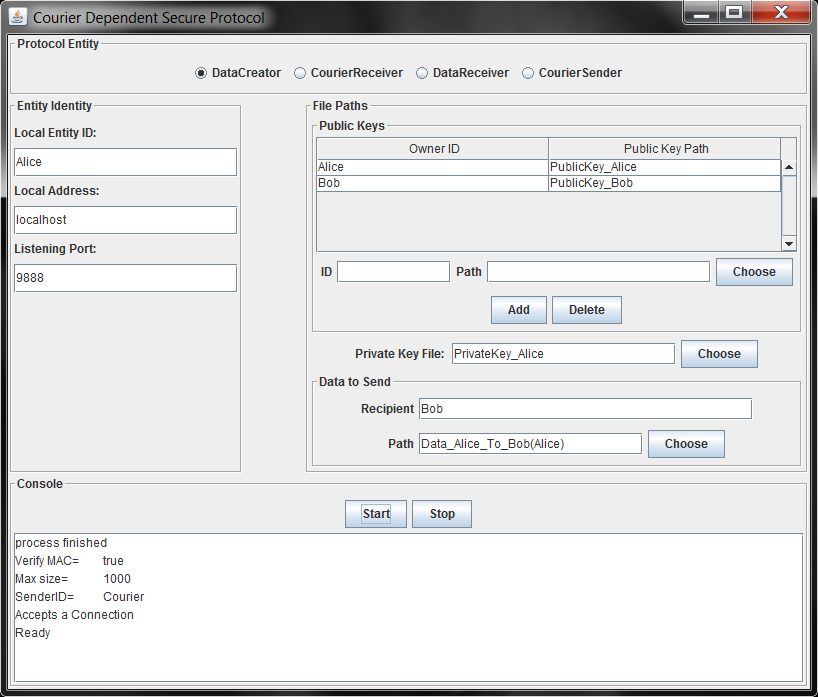
\includegraphics[width=\textwidth,natwidth=818,natheight=697]{figures/GUIdatacreator.png}
  \caption{DataCreator}
 \end{subfigure}
 \begin{subfigure}[b]{0.49\textwidth}
  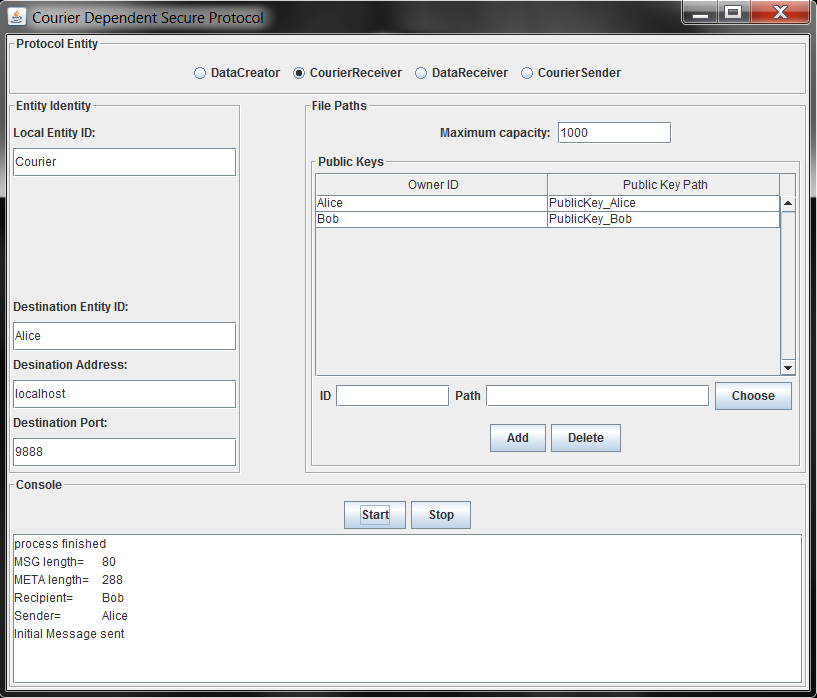
\includegraphics[width=\textwidth,natwidth=817,natheight=698]{figures/GUIcourierreceiver.png}
  \caption{CourierReceiver}
 \end{subfigure}
 \caption{Running Submit Protocol} 
\end{figure}

\subsubsection{Run Transmit Protocol}
It requires at least 2 devices to run this protocol, we call them $ D_1 $ and $ D_2 $. Assume $ D_1 $ is entity Courier, who possesses an encrypted message from Alice and wants to send it to Bob. Assume $ D_2 $ is entity Bob, who waits to receive message from Alice. The running procedure of Transmit Protocol is:

\begin{enumerate}
\item $ D_2 $ starts the application.

\item $ D_2 $ user selects ``DataReceiver" in the Protocol Entity panel.

\item $ D_2 $ user specifies the entity ID, local address and listening port (8888 by default) by filling the corresponding textfields in Entity Identity panel.

\item $ D_2 $ user adds destination entity's public key into its public key list. The way of doing that has been introduced in the step 4 of running Submit Protocol.

\item $ D_2 $ user specifies its private key by filling the textfield with the private key file.

\item $ D_2 $ user click Start button in the Console panel. The running progress of the protocol will be displayed in the information board in the Console panel.

\item $ D_1 $ starts the application.

\item $ D_1 $ user selects ``CourierSender" in the Protocol Entity panel.

\item $ D_1 $ user specifies its own entity ID by filling the textfield in Entitiy Identity panel.

\item $ D_1 $ user specifies the ID of the entity he wants to contact (here $ D_2 $'s ID), together with its address and port number by filling corresponding textfields in the rest of Entity Identity panel.

\item $ D_1 $ user add the public key of the entity he wants to contact into the public key list. The way of doing that has been introduced in step 4.

\item $ D_1 $ user specifies the file that contains the data needs to be sent, by filling the file path in the corresponding textfield in Data to Send panel.

\item $ D_1 $ user click the Start button in the Console panel. The running progress of the protocol will be displayed in the information board in the Console panel.
\end{enumerate}
Below figures show snapshot of two applications successfully running Transmit Protocol. After application consoles on both devices pops ``process finish" successfully, the data carried by $ D_1 $ has been transmitted to $ D_2 $. If the authenticity of the data is successfully verified, $ D_2 $ will print the message content out in the information board. If the data contains messages from multiple senders, they will be verified and printed one by one so that user knows which messages have been discarded.

\begin{figure}[!h]
 \centering
 \begin{subfigure}[b]{0.49\textwidth}
  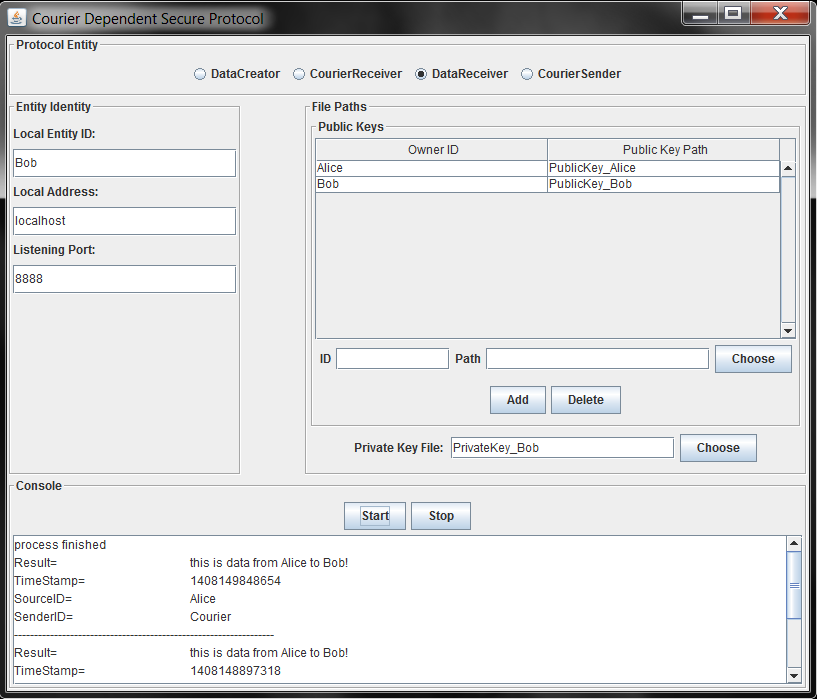
\includegraphics[width=\textwidth,natwidth=818,natheight=697]{figures/GUIdatareceiver.png}
  \caption{DataReceiver}
 \end{subfigure}
 \begin{subfigure}[b]{0.49\textwidth}
  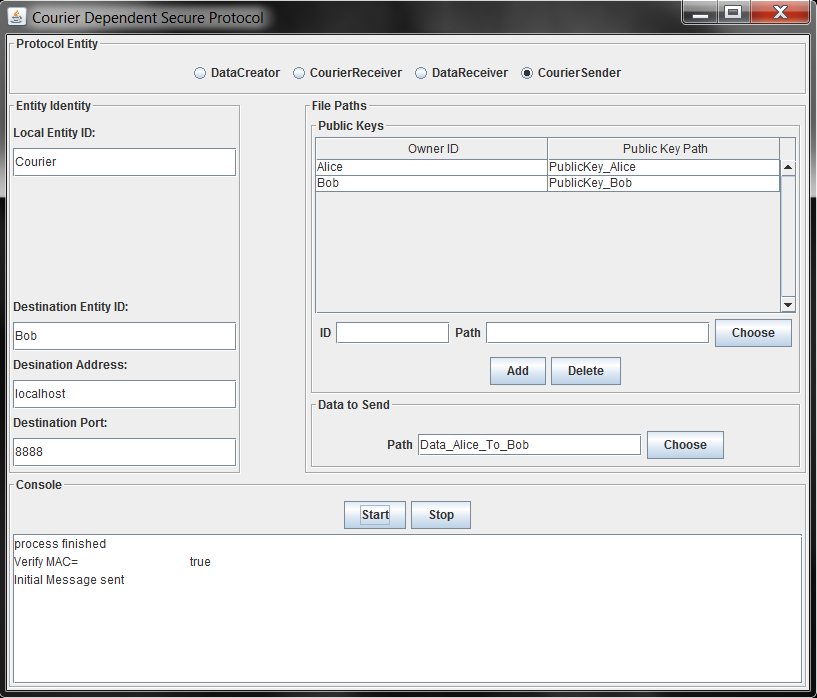
\includegraphics[width=\textwidth,natwidth=817,natheight=698]{figures/GUIcouriersender.png}
  \caption{CourierSender}
 \end{subfigure}
 \caption{Running Submit Protocol} 
\end{figure}

\subsubsection{Use Case}


\subsection{Software Design}
The implementation of this protocol mainly consists of two parts - a core library and an user interface. The core library defines the framework of the program and provides all essential components for running the protocol. While the user interface takes user's input, configures components provided by the core library, runs the protocol and outputs running results if necessary. This design separates the implementation of user interfaces from the actual running of the protocol, the major benefit is that when this protocol is running on different devices or platforms, various user interfaces can be created and easily plugged to the protocol library without modifying the core library.

\subsubsection{Program Architecture}
\paragraph{Framework}
\paragraph{Entity Model}
The $\mathcal{S}$ denotes its set of internal states which defines how $\prod$ responds to a certain input $\mathcal{M}$. Taking $\mathcal{A}$ as example,the figure below shows a 3-internal-state oracle which abstracts the behaviour of $\mathcal{A}$: initially $\prod_S$ is in Wait state, waiting for incoming message
. Once it receives and verifies $\mathcal{M}_0$, it sends the $\mathcal{M}_0'$ out and enters Send state, waiting for next message. After that it receives and verifies  $\mathcal{M}_1$ and enters the final state Check. If any error occurs when $\prod_S$ in Wait or Send state, it enters Error state and session is aborted.

\begin{figure}[h!]
\centering
\includegraphics[width=0.8\textwidth,natwidth=585,natheight=298]{figures/statemachinefigure.png}
\caption{State Machine Model}
\end{figure}

\subsubsection{Message Structure}

\subsection{Implementation Details}
\paragraph{UML Class Diagram}
